\newpage
\section{Architettura}
In questa breve sezione, viene fornita una visione ad alto livello dell'intera architettura del prodotto \progetto, ovvero come sono strutturati e suddivisi i packages più importanti, mettendo in evidenza la separazione tra \textit{front-end\ped{G}} e \textit{back-end\ped{G}}.

\subsection{Visione ad alto livello}
Il software API Market implementa una classica applicazione \textit{Client-Server}, caratterizzata da un lato \textit{front-end\ped{G}} (Client), il quale si occuperà di fornire all'utente della piattaforma l'interfaccia web su cui poter interagire, e un lato \textit{back-end\ped{G}} (Server) che avrà il compito di reperire, salvare e fornire dati, e, tramite l'opportuna componente \textit{API Gateway}, si occuperà della gestione delle chiamate ai microservizi disponibili. Le basi di dati utilizzate, si occuperanno della raccolta di dati sensibili dell'utenza, della gestione dei microservizi e delle relative chiavi e, infine, dell'elaborazione dei dati statistici in merito alla \textit{SLA\ped{G}}.
Per il lato front-end, verrà utilizzato il framework \textit{Angular 2\ped{G}}, unito ai comuni linguaggi \textit{HTML5\ped{G}}, \textit{CSS3\ped{G}} e \textit{JavaScript\ped{G}}.
Per il lato back-end, invece, verrà utilizzato il linguaggio Jolie per la realizzazione di microservizi per l'interfacciamento con le basi di dati e con l'API Gateway; quest'ultimo, infine, sarà implementato tramite i linguaggi Jolie e Java.

\begin{figure}[H]
	\centering
	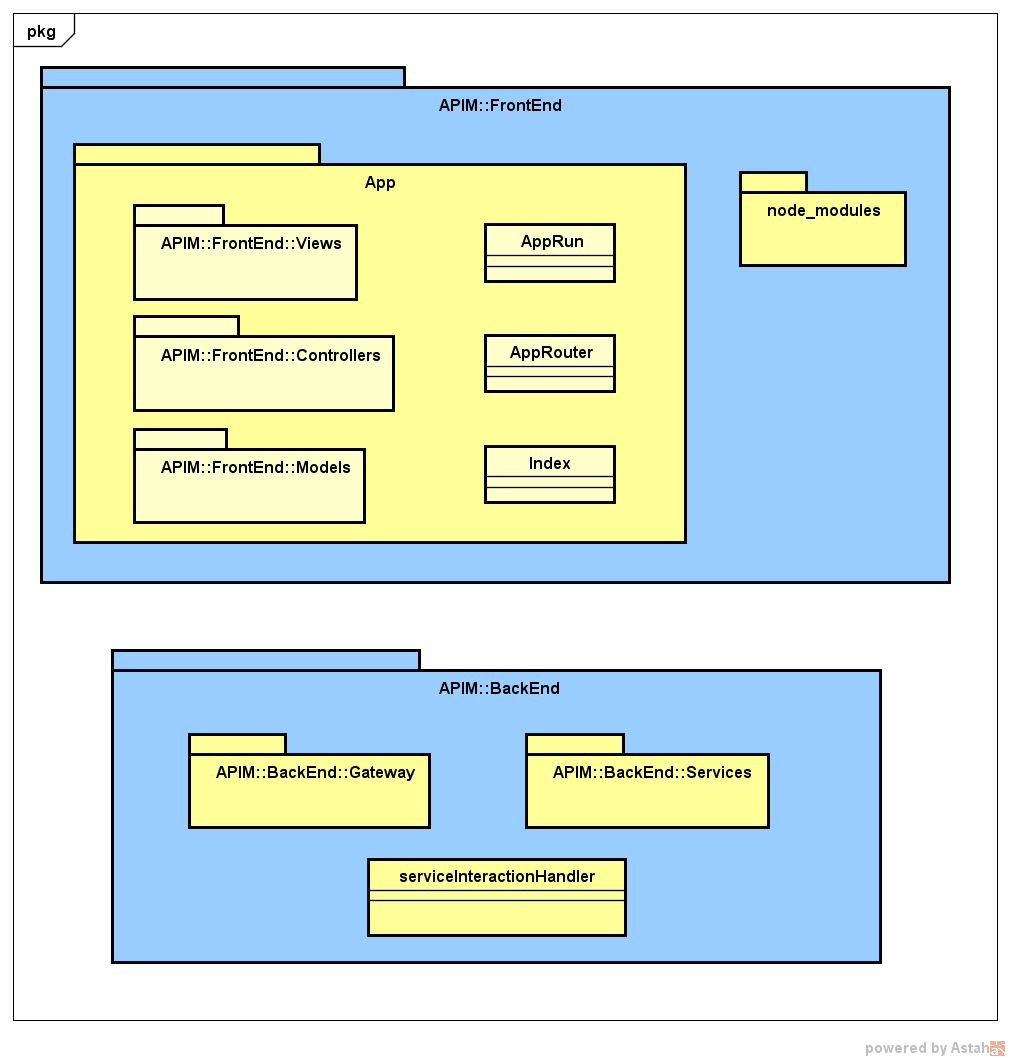
\includegraphics
	[width=0.7\linewidth]
	{images/APIM/Architettura_generale.png}
	\caption{Architettura generale}
\end{figure}

\subsubsection{Informazioni generali}
Di seguito, sono raccolte le informazioni generali dello schema presentato precedentemente:
	\begin{itemize}
		\item \textbf{Descrizione:} architettura ad alto livello della piattaforma \progetto.
		\item \textbf{Packages contenuti:}
		\begin{itemize}
			\item APIM::FrontEnd: package contenente tutti i packages che compongono la parte di front-end dell'applicazione;
			\item APIM::BackEnd: package contenente tutti i packages che compongono la parte di back-end dell'applicazione.
		\end{itemize}
	\end{itemize}
